% rf_channels.tex — ONE source, ONE rendered SVG (rf_channels.svg), embedded in
% ../rfdc/channels.md under "## One port per channel".
%
% The claim, and it is an ASYMMETRY claim rather than an interface one: the two sides of a converter
% count channels differently on purpose.  The fabric side gets `n_rx` + `n_tx` SEPARATE AXI-Stream
% ports, one per channel, because that is what the IP presents and because one wide interleaved port
% would push a vendor packing rule into every design.  The RF side gets ONE RFSampIF per direction
% carrying every channel of that direction in a single (n_ch, blksize) block, because the RF
% environment and the user's logic both want the channels together — splitting it would give n_ch
% events per block period, against the whole point of block-rate modelling.
%
% Distinct from rf_interfaces.tex, which names the four endpoints of a ONE-channel converter.  This
% one is about how those endpoints multiply (or do not) as channels are added.
%
% Render: bash render.sh   (MiKTeX pdflatex -> PDF -> dvisvgm --pdf -> SVG)
\documentclass[tikz,border=4pt]{standalone}
\usepackage{tikz}
\usetikzlibrary{arrows.meta,positioning,calc,fit,backgrounds}

\definecolor{nyuviolet}{HTML}{57068C}
\definecolor{nyuultra}{HTML}{330662}
\definecolor{nyupale}{HTML}{EFE6F5}
\definecolor{nyumid}{HTML}{8A5FB0}
\definecolor{envfill}{HTML}{F1EFF3}
\definecolor{envline}{HTML}{6E6A73}
\definecolor{inkgray}{HTML}{444444}

\begin{document}
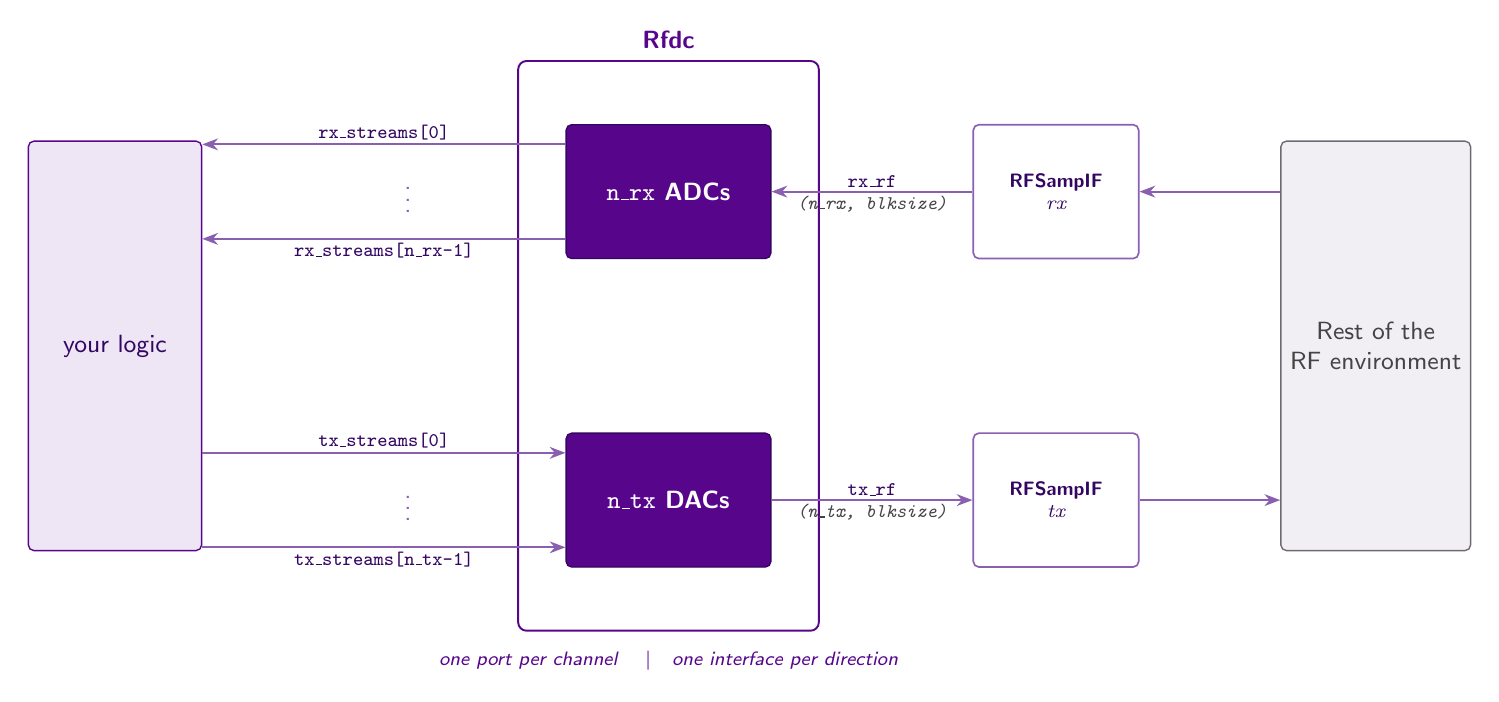
\begin{tikzpicture}[
  font=\sffamily\small,
  fab/.style  = {draw=nyuviolet, line width=0.5pt, fill=nyupale, rounded corners=2pt,
                 minimum width=22mm, minimum height=52mm, text=nyuultra, align=center},
  env/.style  = {draw=envline, line width=0.5pt, fill=envfill, rounded corners=2pt,
                 minimum width=24mm, minimum height=52mm, text=inkgray, align=center},
  core/.style = {draw=nyuultra, line width=0.5pt, fill=nyuviolet, rounded corners=2pt,
                 minimum width=26mm, minimum height=17mm, text=white,
                 font=\sffamily\small\bfseries, align=center},
  ifb/.style  = {draw=nyumid, line width=0.6pt, fill=white, rounded corners=2pt,
                 minimum width=21mm, minimum height=17mm, text=nyuultra,
                 font=\sffamily\scriptsize\bfseries, align=center},
  box/.style  = {draw=nyuviolet, line width=0.7pt, fill=white, rounded corners=3pt},
  ln/.style   = {-{Stealth[length=2mm]}, draw=nyumid, line width=0.7pt},
  lbl/.style  = {font=\sffamily\scriptsize, text=nyuultra, inner sep=1.2pt},
  sub/.style  = {font=\sffamily\scriptsize\itshape, text=inkgray, inner sep=1.1pt},
  dots/.style = {font=\sffamily\small, text=nyumid, inner sep=0.5pt},
]

% --- the converter, and its two blocks -----------------------------------------------------------
\node[core] (adc) {\texttt{n\_rx} ADCs};
\node[core, below=22mm of adc] (dac) {\texttt{n\_tx} DACs};
\begin{scope}[on background layer]
  \node[box, fit=(adc)(dac), inner xsep=6mm, inner ysep=8mm] (rfdc) {};
\end{scope}
\node[lbl, font=\sffamily\small\bfseries, text=nyuviolet, above=1mm of rfdc.north] {Rfdc};

% --- the two sides -------------------------------------------------------------------------------
\node[fab, left=40mm of rfdc] (dut) {your logic};

\node[ifb] (rxif) at ([xshift=30mm]rfdc.east |- adc) {RFSampIF\\\normalfont\itshape rx};
\node[ifb] (txif) at ([xshift=30mm]rfdc.east |- dac) {RFSampIF\\\normalfont\itshape tx};
\node[env] (env) at ([xshift=30mm]$(rxif.east)!0.5!(txif.east)$)
  {Rest of the\\RF environment};

% --- fabric side: ONE PORT PER CHANNEL, drawn as separate lines -----------------------------------
% RX: the ADCs drive n_rx master ports, right to left.
\coordinate (rx0) at ([yshift=6mm]adc.west);
\coordinate (rxN) at ([yshift=-6mm]adc.west);
\draw[ln] (rx0) -- node[lbl, above] {\texttt{rx\_streams[0]}}      (rx0 -| dut.east);
\draw[ln] (rxN) -- node[lbl, below] {\texttt{rx\_streams[n\_rx-1]}} (rxN -| dut.east);
\node[dots] at ($(rx0)!0.5!(rxN) + (-20mm,0)$) {$\vdots$};

% TX: your logic drives n_tx slave ports, left to right.
\coordinate (tx0) at ([yshift=6mm]dac.west);
\coordinate (txN) at ([yshift=-6mm]dac.west);
\draw[ln] (tx0 -| dut.east) -- node[lbl, above] {\texttt{tx\_streams[0]}}      (tx0);
\draw[ln] (txN -| dut.east) -- node[lbl, below] {\texttt{tx\_streams[n\_tx-1]}} (txN);
\node[dots] at ($(tx0)!0.5!(txN) + (-20mm,0)$) {$\vdots$};

% --- RF side: ONE interface per direction, carrying every channel ---------------------------------
\draw[ln] (rxif.west) -- node[lbl, above] {\texttt{rx\_rf}}
                         node[sub, below] {\texttt{(n\_rx, blksize)}} (adc.east);
\draw[ln] (dac.east) -- node[lbl, above] {\texttt{tx\_rf}}
                        node[sub, below] {\texttt{(n\_tx, blksize)}} (txif.west);

\draw[ln] (env.west |- rxif) -- (rxif.east);
\draw[ln] (txif.east) -- (env.west |- txif);

% --- the asymmetry, named -------------------------------------------------------------------------
\node[sub, below=2mm of rfdc.south, text=nyuviolet, align=center]
  {one port per channel \quad$\vert$\quad one interface per direction};

\end{tikzpicture}
\end{document}
